\subsection{Main Survey Questions}
\label{appdx:survey}

% \todo{Let's remove "examples" from the section title and add all questions below along with the type of responses (text, likert, multiple choice, etc.)}

% \begin{figure}[h!]
%     \centering
%     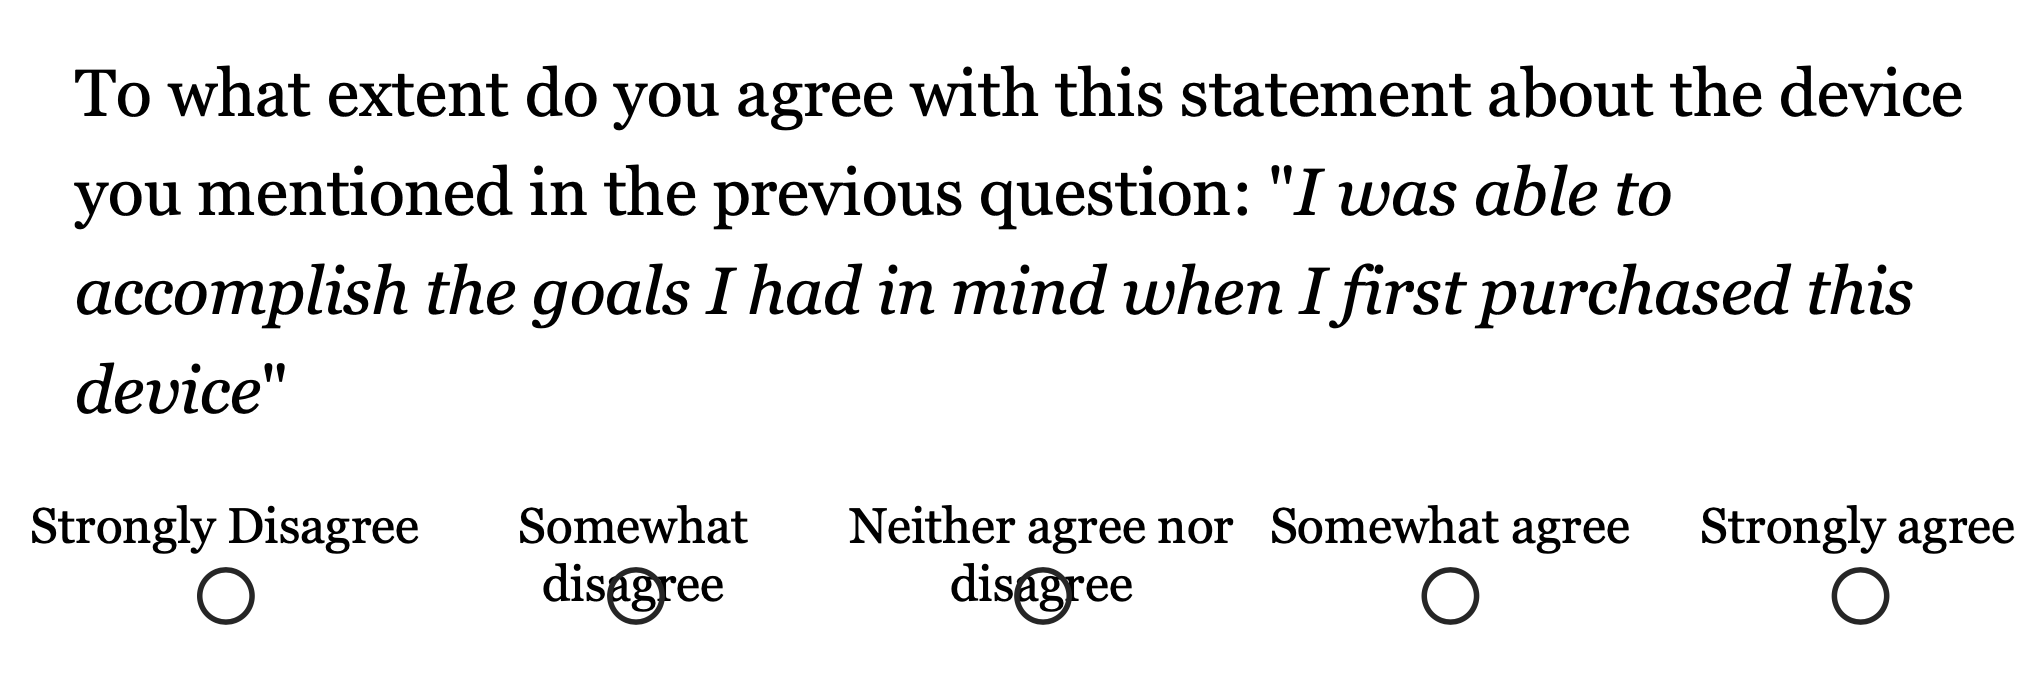
\includegraphics[width=0.8\linewidth]{text/appendix/likert.png}
% \end{figure}

% \begin{figure}[h!]
%     \centering
%     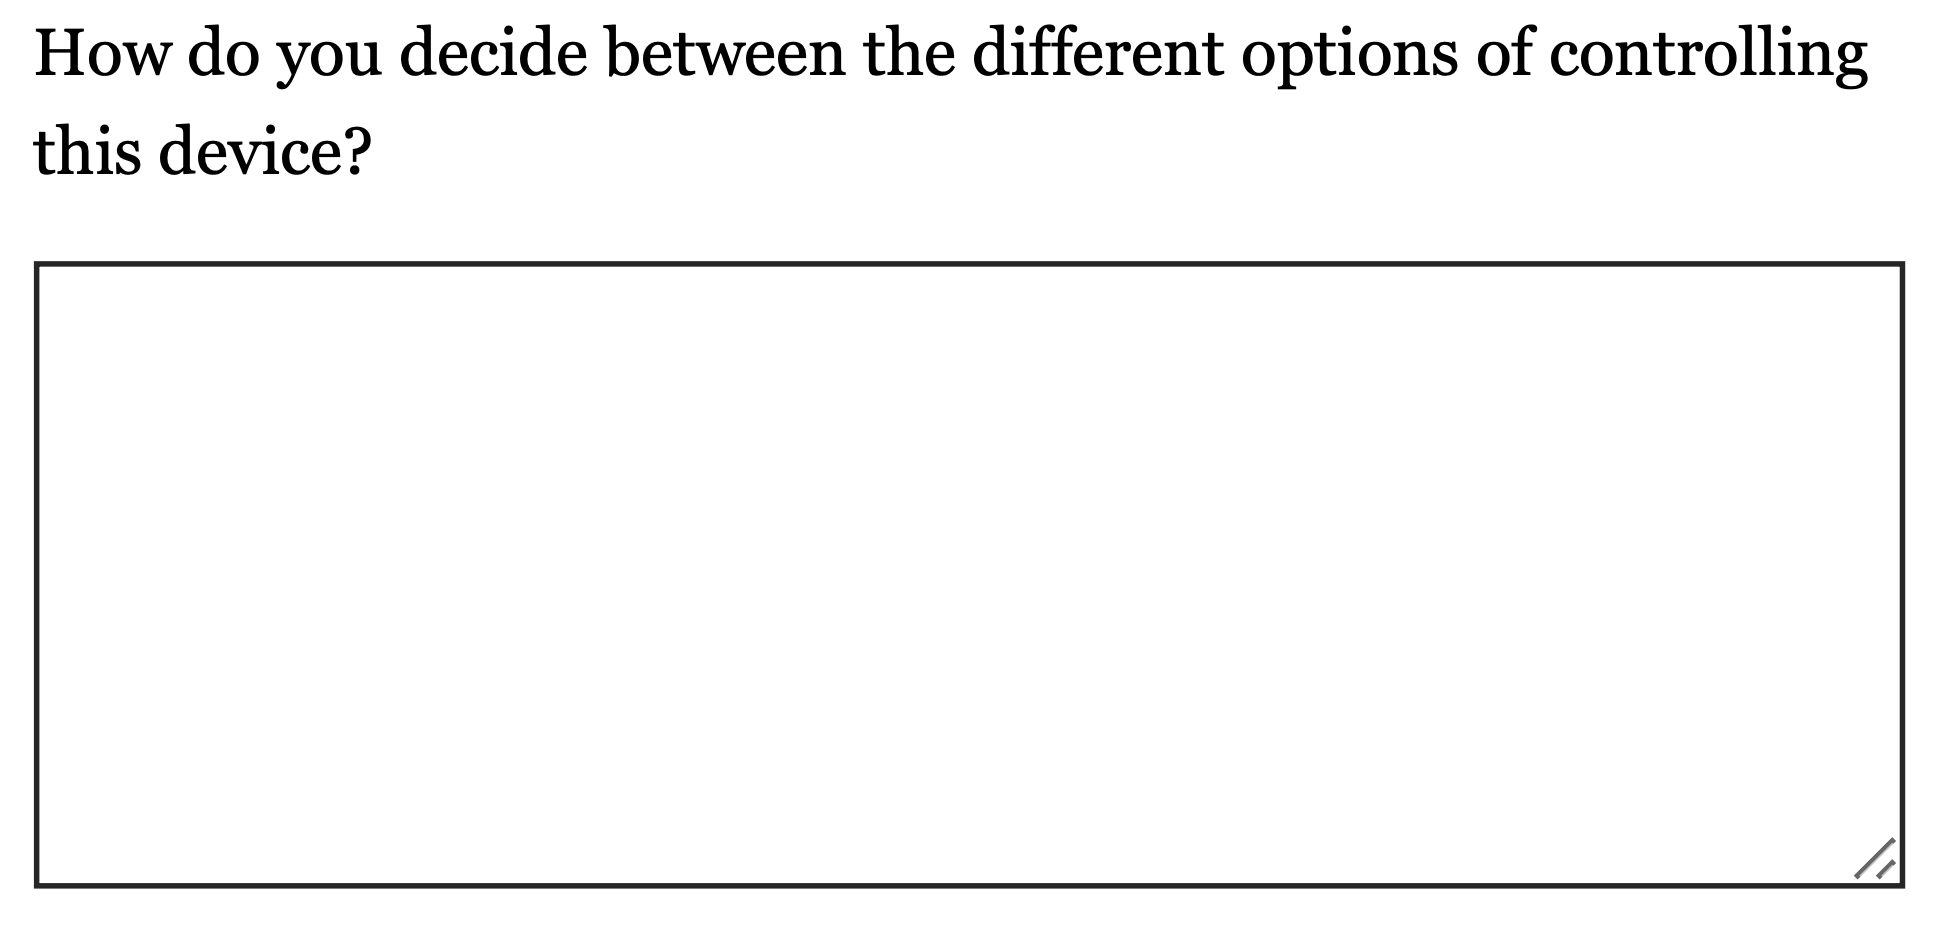
\includegraphics[width=0.8\linewidth]{text/appendix/free_response.png}
% \end{figure}

% \begin{figure}[h!]
%     \centering
%     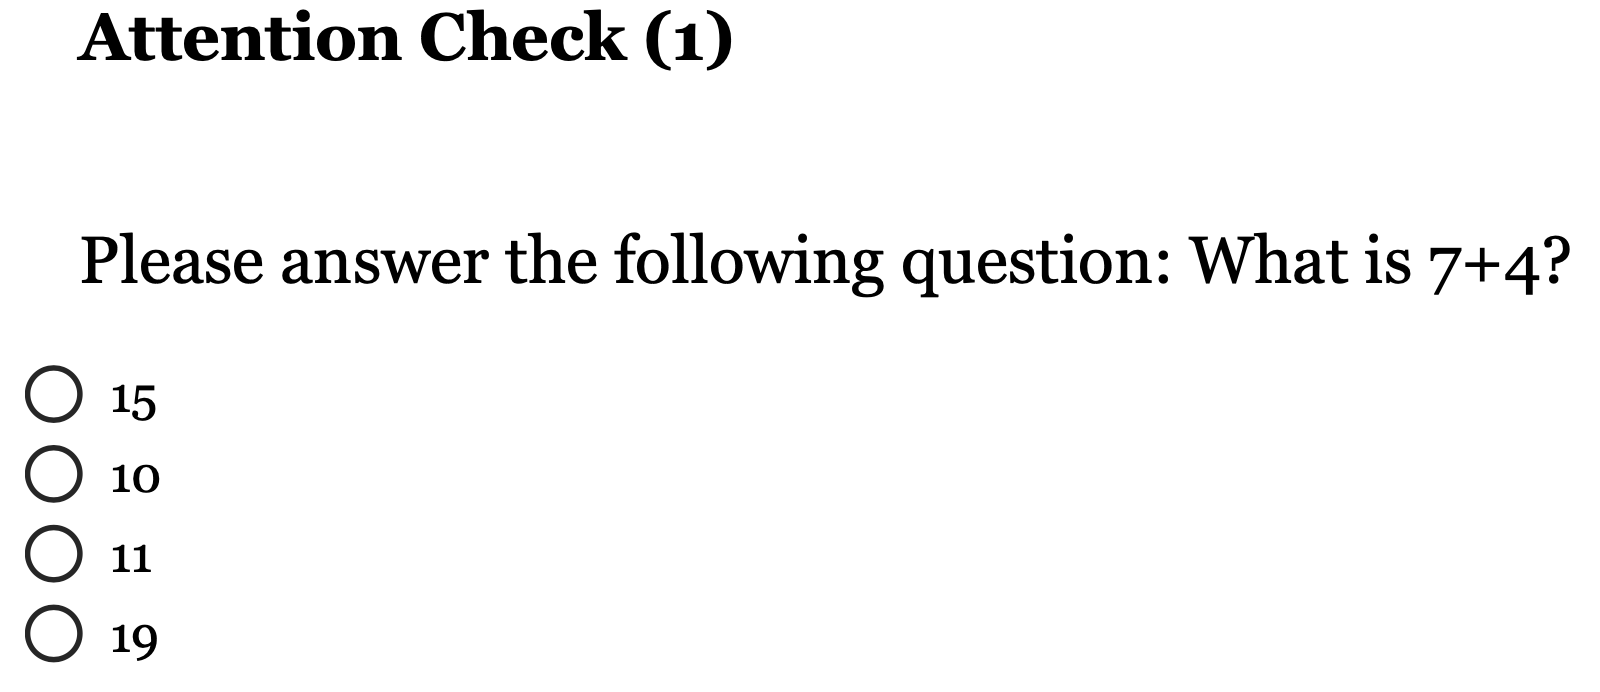
\includegraphics[width=0.8\linewidth]{text/appendix/attention_check.png}
% \end{figure}

\subsubsection{Consent Block}
\label{appdx:survey:consent}

\printQcounter{} You are being asked to participate in a voluntary research study. The purpose of this study is to build a taxonomy of smart home user workloads and failures for both centralized (using a smart home hub) and per-device control schemes. Your responses will provide us with information regarding existing approaches to controlling smart home device infrastructures, and the reasons for opting to use certain control schemes.

Participating in this study will involve answering a set of survey questions about your experiences and current smart home setups. Participation will last approximately 20 minutes. We will not be asking you to use any of these devices in front of us, but instead we will be asking you to recount experiences with these devices. There are no foreseeable risks to you beyond those normally encountered in your daily life while participating in this survey. If you agree to participate, you will be asked to check "I consent" at the bottom of this page indicating that you have read the following form and have been shown the goals of this study.

Principal Investigator Name and Title: Removed for anonymity

What procedures are involved?
The study procedures are an online survey that you will be asked to complete. In this survey, you will be asked about your smart home setup, including the kinds of devices you own and use, as well as how you control them. We will then ask some questions about specific experiences with these devices, and how these experiences have affected your perception of these devices and corresponding control schemes.

This research will be performed online, using an online survey software (Qualtrics). Participation will consist of one single survey, that will take approximately 20 minutes to complete.

Will my study-related information be kept confidential?
We will use all reasonable efforts to keep your personal information confidential, but we cannot guarantee absolute confidentiality. When this research is discussed or published, no one will know that you were in the study. But, when required by law, identifying information may be seen or copied by: a) The Institutional Review Board that approves research studies; b) The Office for Protection of Research Subjects and other university departments that oversee human subjects research; c) University and state auditors responsible for oversight of research.

Will I be reimbursed for any expenses or paid for my participation in this research?
You will be compensated 4\$ USD upon completion of this survey.

Can I withdraw or be removed from the study?
If you decide to participate, you are free to withdraw your consent and discontinue participation at any time. Your participation in this research is voluntary. Your decision whether to participate, or to withdraw after beginning participation, will not affect your current or future dealings with [Removed for Anonymity]. 

The researchers also have the right to stop your participation in this study without your consent if they believe it is in your best interests, you were to object to any future changes that may be made in the study plan.

Will data collected from me be used for any other research?
Your de-identified information could be used for future research without additional informed consent.

Who should I contact if I have questions?
Removed for anonymity

What are my rights as a research subject?
Removed for anonymity

Please print this consent form if you would like to retain a copy for your records.

I have read and understand the above consent form. I certify that I am 18 years old or older. By clicking the “I consent” button to enter the survey, I indicate my willingness to voluntarily take part in this study. \\
\textit{Answer type:} Multiple choice. Options were: ``I consent.'' and ``I do not consent.'' If a participant chose ``I do not consent.'' they were automatically redirected to the end of the survey.

\subsubsection{Screening Block}
\label{appdx:survey:screen}

\printQcounter{} How many Smart Devices do you currently own? As a reminder, Smart Devices are defined as: Everyday objects made intelligent with network capabilities to execute tasks either automatically or on demand. Some examples of these devices are, but not limited to: smart plugs/switches, smart lights, smart door locks, smart thermostats, smart vacuums, window/door sensors, motion sensors, smart smoke alarms, smart cameras/security systems, smart TVs, smart speakers (amazon echo, google home), etc. Excludes smartphones, tablets, computers.\\
\textit{Answer type:} Multiple choice. Options were: ``I do not own any dmart devices'', ``1'', ``2'', ``3'', ``4'', ``5 or more smart devices''.

\subsubsection{Intro Block}
\label{appdx:survey:intro}
Thank you for participating in this survey. The purpose of this survey is to understand user experiences and perceptions with smart home device control, and how these perceptions change over time. Your responses will provide valuable information to help answer our research questions. Please keep in mind that this survey is not a test of your knowledge, but a way to learn about your experiences; there are no right or wrong answers.

For your reference, here are some definitions to terms you may encounter in this survey:
 
Smart Devices: Everyday objects made intelligent with network capabilities to execute tasks either automatically or on demand. Some examples of these devices are, but not limited to: smart plugs/switches, smart lights, smart door locks, smart thermostats, smart vacuums, window/door sensors, motion sensors, smart smoke alarms, smart cameras/security systems, smart TVs, smart speakers (amazon echo, google home), etc. Excludes smartphones, tablets, computers.
 
Smart Device Control: The ability to view and change the current state of a smart device. The smart device itself, a physical controller or an application may be access points to control the smart device. Typically, smart devices are paired with the control medium, if that is different from the device itself, before the user can control the device. For example, you can control a smart lock on the front door either directly or with your phone. 

For the purposes of this study, we will differentiate between different ways you may control your smart home devices:

Centralized Control: Control of multiple smart devices from a central service (e.g., digital twin) or device (e.g.,  smart hub), that has a global view of all devices' states and access to modify the state of any and all of the devices. All smart devices must initially be paired with the central service by the user. Some examples of centralized controllers are: Amazon Echo, Google Home mini, Apple HomePod for devices, and Amazon Alexa, Google Home, Google Assistant and Apple HomeKit for applications.

Per-device control: Control of smart devices by pushing or rotating buttons on an individual device itself or by using an application that the device vendor has provided the customers. The user must pair the smart device with the device vendor if they desire controlling it by the provided app. Some examples of per-device controllers include but are not limited to: Philips Hue Bridge, Wink+GE In-Wall Smart Switch for devices, Philips Hue, ecobee for applications.

Routine: An automation that involves smart devices. A set of actions, and potentially a set of triggering conditions, are specified. Each action changes the current state of a smart device. Each triggering condition checks the current state of a smart device or the current date and time; triggering conditions may be combined with a conjunction or a disjunction. A routine may also be manually triggered by a user, rather than triggering clauses. Other names for a routine in current products are: recipe, scene, schedule.

Lastly, we define the following term(s):

Troubleshooting: Tracing and correcting faults in a mechanical or electronic system. An example of a troubleshooting process is the following:

\begin{enumerate}
    \item You are at home and your smart vacuum no longer responds to your control through your Amazon Echo device.
    \item You check that your smart vacuum base is connected to a power outlet; it is.
    \item You check that your smart vacuum is connected to the WiFi in your home; it is.
    \item You check that your smart phone has access to the internet when connected through the home WiFi; it does not.
    \item You check that your home router has access to the internet; it does not.
    \item You reboot your home router and wait for 5 minutes.
    \item Your smart vacuum responds to your commands through your Amazon Echo device.
\end{enumerate}

Please remember that you are answering on behalf of your household.

\printQcounter{} Please enter your prolific ID.\\
\textit{Answer type:} Text entry (single line).

\subsubsection{General Smart Home Setup Questions}
\label{appdx:survey:general}

\printQcounter{} Which of the following smart home devices do you have powered on where you are living now? In the first column, select all that apply. For each owned device, in the second column, write how many you own and in the third column check each location in the home where you have the device. Finally, in the fourth column, describe the device's primary use in your home. 

Recall that smart devices are defined as: "Everyday objects made intelligent with network capabilities to execute tasks either automatically or on demand."
If you are at home, feel free to walk around and look at devices to jog your memory.\\
\textit{Answer type:} Table filling. Each row represented a smart device kind out of plug/switch, light, lock, thermostat, vacuum/mop, window/door sensor, motion sensor, smoke alarm, camera, security system, TV/casting device, speaker, tag, health device, washing machine/dryer, dishwasher, fridge, coffee maker, oven/range, trash can, other. There was a row for "I do not own any smart devices" as well. Each device kind was accompanied by a couple of representative devices. The first column had checkmarks to be clicked if a device kind was owned. The second column asked for the number of owned devices for each device kind. Next, we asked in a separate group of columns for participants to pick the spaces their devices of each kind were located at in their home; options were: entrance hall, living room, dining room, kitchen, master bedroom, children's bedroom, guestroom, study, wardrobe, bathroom, basement, laundry room, hallway, entertainment/game room, attic, garage, porch (front/back), yard/garden/pool, driveway, and other. The final column asked participants for the primary use of the device kind.

\printQcounter{} If you selected other, for each device:
Please list the number of devices, their type, their location in your home, and their main use. \\
\textit{Answer type:} Text entry (multiple lines).

\printQcounter{appno} Look at your phone. How many smart home device related applications do you have installed on your phone? \\
\textit{Answer type:} Multiple choice. Options were: ``0'', ``1-4'', ``5-8'', ``More than 8''.

% \noindent \textit{If Q5 answer was not ``0'':}
\printQPrefix{If Q\ref{appno} answer was not ``0''} Please list the smart home device related applications on your phone.\\
\textit{Answer type:} Text entry (essay text box).

\printQcounter{} When was the last time you purchased a smart device for your home? \\
\textit{Answer type:} Multiple choice. Options were: ``Less than one month ago'', ``Less than six months ago'', ``Less than one year ago'', and ``More than one year ago''.

\printQcounter{} What was one of the last smart devices you purchased for your home? Why did you purchase it? \\
\textit{Answer type:} Text entry (essay text box).

\printQcounter{} To what extent do you agree with this statement about the device you mentioned in the previous question: "I was able to accomplish the goals I had in mind when I first purchased this device"? \\
\textit{Answer type:} Multiple choice. Options were: ``Strongly disagree'', ``Somewhat disagree'', ``Neither agree nor disagree'', ``Somewhat agree'', and ``Strongly agree''.

\printQcounter{} For any goal that you were not able to accomplish, please list the reasons. \\
\textit{Answer type:} Text entry (essay text box).

\printQcounter{} For any goal that you were able to accomplish, please tell us how you reached them. \\
\textit{Answer type:} Text entry (essay text box).

\subsubsection{Attention Check (1)}

\printQcounter{} Please answer the following question: What is 7+4? \\
\textit{Answer type:} Multiple choice. Options were: ``15'', ``10'', ``11'', and ``19''.

\subsubsection{Device Control Questions}
\label{appdx:survey:control}

\printQcounter{} Pick a specific device in your home, and write down that device below.\\
\textit{Answer type:} Text entry (single line).

The next few questions deal with this device that you mentioned above.

\printQcounter{} How often is the device you listed above in use (manually or via automation)? \\
\textit{Answer type:} Multiple choice. Options were: ``At least three times a week'', ``At least once a week'', ``At least once a month'', and ``Only a couple times since I got it''.

\printQcounter{} What is the way the device you listed above is most commonly used? \\
\textit{Answer type:} Multiple choice (multiple answers allowed). Options were: ``Routines (defined as 'An automation that involves smart devices. A set of actions, and potentially a set of triggering conditions, are specified. Each action changes the current state of a smart device`, ``Central Control (defined as 'Control of smart devices from a central service (e.g., digital twin) or device (e.g., smart hub), that has a global view of all devices' states and access to modify the state of any and all of the devices.`)'', ``Per-Device Control (defined as 'Control of smart devices by pushing or rotating buttons on an individual device itself or by using an application that the device vendor has provided the customers.`)'', ``Voice Command'' and ``Content streaming casting''.

\printQcounter{} Why do you choose to control the device you listed above this way(s)? \\
\textit{Answer type:} Text entry (essay text box).

\printQcounter{multischeme} Is there any device in your home that can be controlled in multiple ways? (this can be the same device that you talked about on the previous page)\\
\textit{Answer type:} Multiple choice. Options were: ``No'', ``Yes'', and ``I don't remember''.

\printQPrefix{If Q\ref{multischeme} answer was ``Yes''} If there are multiple devices that can be controlled in multiple ways, think about one of these devices. What device is that? \\
\textit{Answer type:} Text entry (essay text box).

\printQPrefix{If Q\ref{multischeme} answer was ``Yes''} How do you decide between the different options of controlling this device? \\
\textit{Answer type:} Text entry (essay text box).

\printQcounter{central} Are you aware that central smart home managers exist? Examples include Amazon Alexa, Google Home, Apple Home.\\
\textit{Answer type:} Multiple choice. Options were: ``Yes'' and ``No''.

\printQPrefix{If Q\ref{central} answer was ``Yes''} How did you learn about central smart home managers? \\
\textit{Answer type:} Multiple choice (multiple answers allowed). Options were: ``Internet'', ``Social media'', ``Streaming services'', ``Physical/Online stores'', ``Word of mouth'', and ``Other (please specify)'' with a text box next to it.

\subsubsection{Device Exceptions (Blame Placement) Questions}
\label{appdx:survey:exceptions}

\printQcounter{exception} Have you had any experience(s) when one or more of your smart devices did not work as planned? \\
\textit{Answer type:} Multiple choice. Options were: ``No'', ``Yes'', and ``I don't remember''.

\printQPrefix{If Q\ref{exception} answer was ``Yes''} Can you describe an experience from a specific time when things didn't go as planned? \\
\textit{Answer type:} Text entry (essay text box).

\printQPrefix[experience]{If Q\ref{exception} answer was ``Yes''} Which of the following statements represents your current experiences with smart devices?
\textit{Answer type:} Multiple choice. Options where: ``I am having the same kinds of issues again and again'', ``I encounter a specific kind of issue just once and the next ones are unrelated'', ``I don't remember if there are patterns among the issues I come across'', and ``I am not encountering any issues with my smart devices''.

\printQPrefix{If Q\ref{exception} answer was ``Yes'' and Q\ref{experience} answer was not ``I am not encountering any issues with my smart devices''} What was your reaction to any smart device failures when you started noticing them? Can you describe the reasons that caused this reaction? \\
\textit{Answer type:} Text entry (essay text box).

\printQcounter{return} Have you ever returned or stopped using a smart device because it didn't work the way you planned? \\
\textit{Answer type:} Multiple choice. Options were: ``No'', ``Yes'', and ``I don't remember''.

\printQPrefix{If Q\ref{return} answer was ``Yes''} What smart devices did you ever return or stop using? \\
\textit{Answer type:} Text entry (essay text box).

\subsubsection{Troubleshooting Questions}
\label{appdx:survey:tb}

\printQPrefix[response]{If Q\ref{exception} answer was ``Yes''} How did you respond when your device did not work as expected? \\
\textit{Answer type:} Multiple choice (multiple answers allowed). Options were: ``I tried to figure out what went wrong'', ``I tried to fix the issue/prevent it from happening again'', ``I stopped using the device'', ``I gave up on that functionality'', ``I don't remember'', and ``Not applicable''.

\printQPrefix{If Q\ref{response} answer ``I tried to fix the issue/prevent it from happening again'' was selected} Describe your troubleshooting process as a sequence of steps.
Recall that troubleshooting is defined as: "The process of tracing and correcting faults in a mechanical or electronic system." \\
\textit{Answer type:} Text entry (essay text box).

\printQPrefix[giveup]{If Q\ref{exception} answer was ``Yes''} Have you ever given up on using a device in your home? \\
\textit{Answer type:} Multiple choice. Options were: ``No'', ``Yes'', and ``I don't remember''.

\printQPrefix{If Q\ref{giveup} answer was ``Yes''} How did you reach that point? \\
\textit{Answer type:} Text entry (essay text box).

\subsubsection{Attention Check (2)}

\printQcounter{} Please answer the following question: What is 15-11? \\
\textit{Answer type:} Multiple choice. Options were: ``10'', ``4'', ``8'', and ``6''.

\subsubsection{Questions about Other Spaces}
\label{appdx:survey:spaces}

\printQcounter{spaces} Are there any more homes or spaces with smart devices that you are the main maintainer of? If so, how many? \\
\textit{Answer type:} Multiple choice. Options were: ``No'', ``Yes, 1 other space'', and ``Yes, 2 or more other spaces''.

\printQPrefix{If Q\ref{spaces} answer was not ``No''} Can you describe where devices are placed in these spaces?Can you describe where devices are placed in these spaces? \\
\textit{Answer type:} Text entry (multiple lines).

\printQPrefix[similar]{If Q\ref{spaces} answer was not ``No''} Do you think there are any similarities between the different spaces' setups? \\
\textit{Answer type:} Multiple choice. Options were: ``No'', ``Yes'', and ``I don't remember''.

\printQPrefix{If Q\ref{spaces} answer was not ``No'' and Q\ref{similar} answer is not ``I don't remember''} Please explain your answer to the previous question. \\
\textit{Answer type:} Text entry (multiple lines).

\subsubsection{Demographic Block}
\label{appdx:survey:demographics}

\printQcounter{} What is your gender? \\
\textit{Answer type:} Multiple choice. Options were: ``Male'', ``Female'', ``Non-binary/third gender'', ``Prefer not to say'', and ``Prefer to self-describe'' with a text box next to it.

\printQcounter{} How would you describe your current living situation? \\
\textit{Answer type:} Multiple choice. Options were: ``House'', ``Apartment'', ``Condominium'', ``Town Home'', ``Prefer not to say'', and ``Other (please specify)'' with a text box next to it.

\printQcounter{} What is the highest degree or level of school that you have completed? \\
\textit{Answer type:} Multiple choice. Options were: ``Some high school, no diploma'', ``High school graduate, diploma or equivalent (for example: GED)'', ``Some college credit, no degree'', ``Associate's degree'', ``Bachelor's degree'', ``Post-graduate degree'', ``Prefer not to say'', and ``Other (please specify)'' with a text box next to it.

\printQcounter{} What is your race? \\
\textit{Answer type:} Multiple choice. Options were: ``White'', ``Black or African American'', ``American Indian or Alaska Native'', ``Asian'', ``Native Hawaian or Pacific Islander'', and ``Hispanic or Latino''.

\printQcounter{} What is your age? \\
\textit{Answer type:} Multiple choice. Options were: ``less than 18 years old'', ``18-24'', ``25-34'', ``35-44'', ``45-54'', ``55-64'', and ``65+''.

\subsubsection{Interview Interest Block}
\label{appdx:survey:interview}

\printQcounter{} Would you be interested in doing a follow-up interview regarding your smart home device and control experience, for additional compensation? If you indicate you are interested, we will reach out via your prolific ID. \\
\textit{Answer type:} Multiple choice. Options were: ``Yes'' and ``No''.

\subsubsection{End of Survey}
We thank you for your time spent taking this survey.
Your response has been recorded.